\documentclass[aspectratio=169]{beamer}
\usepackage{helvet}
\usepackage{calc}
\usepackage[utf8]{inputenc}
\usepackage[english]{babel}

\usetheme{Ilmenau}

\setbeamercovered{transparent}
\setbeamertemplate{navigation symbols}{}

\usepackage{units}
\usepackage{amsbsy}
\usepackage{amsmath}
\usepackage{amssymb}
\usepackage{graphics}
\usepackage{graphicx}
\usepackage{epsf}
\usepackage{epsfig}
\usepackage{fixmath}
%\usepackage{pgfmath}
\usepackage{wrapfig}


\title{Intro to Prometheus}
\subtitle{With a dash of operations \& observability}
\author{Richard Hartmann \& Frederic Branczyk\\
@TwitchiH \& @fredbrancz}
\date{2018-12-12}


\begin{document}

\section{Introduction}

\subsection{}

\begin{frame}
	\titlepage
\end{frame}

\begin{frame}
	\frametitle{Who are we?}
	\begin{itemize}
		\item Richard "RichiH" Hartmann
		\begin{itemize}
			\item Swiss army chainsaw at SpaceNet
			\item Project lead for building one of the most modern datacenters in Europe
			\item Debian Developer
			\item FOSDEM, DebConf, DENOGx, PromCon staff
			\item Prometheus team member
		\end{itemize}
		\item Frederic Branczyk
		\begin{itemize}
			\item Red Hat (previously CoreOS)
			\item All things Prometheus / Kubernetes
			\item Kubernetes SIG-Instrumentation lead
			\item Prometheus team member
		\end{itemize}
	\end{itemize}
\end{frame}

\begin{frame}
	\frametitle{Time split}
	\begin{enumerate}
		\item 1/3 Prometheus
		\item 1/3 Observability
		\item 1/3 Questions
	\end{enumerate}
\end{frame}

\begin{frame}
	\frametitle{Show of hands}
	\begin{itemize}
		\item Who has heard of Prometheus?
		\item Who is considering to use Prometheus?
		\item Who is POCing Prometheus?
		\item Who uses Prometheus in production?
	\end{itemize}
\end{frame}

\begin{frame}
	\frametitle{Prometheus 101}
	\begin{itemize}
		\item Inspired by Google's Borgmon
		\item Time series database
		\item unit64 millisecond timestamp, float64 value
		\item Instrumentation \& exporters
		\item Not for event logging
		\item Dashboarding via Grafana
	\end{itemize}
\end{frame}


\section{Prometheus}


\subsection{}

\begin{frame}
        \frametitle{Generating, scraping, and persisting times series}
        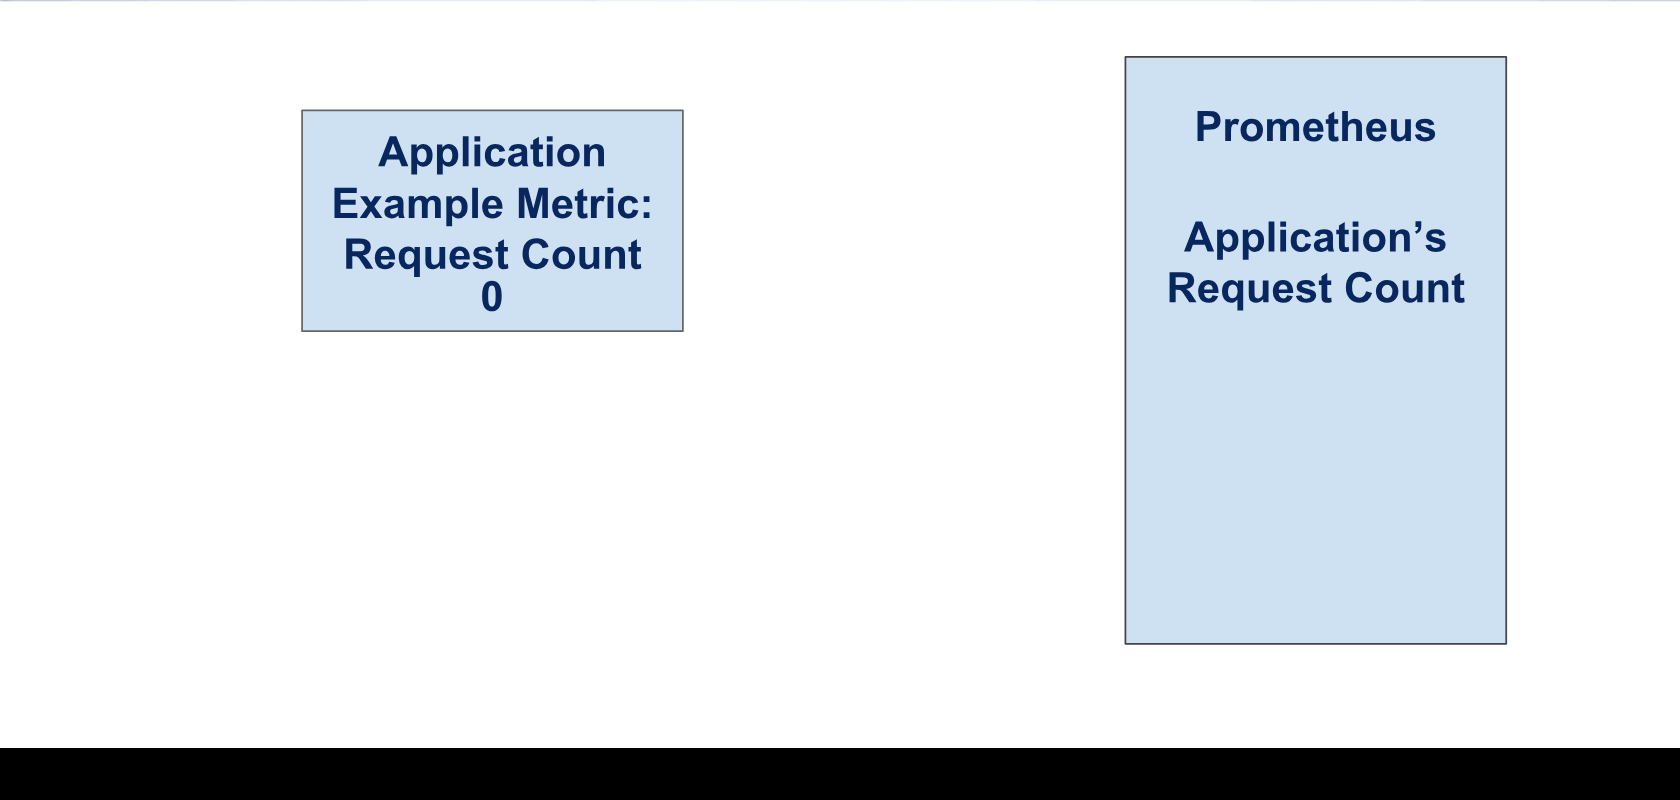
\includegraphics[width=\textwidth]{01-cropped.png}
\end{frame}

\begin{frame}
        \frametitle{Generating, scraping, and persisting times series}
        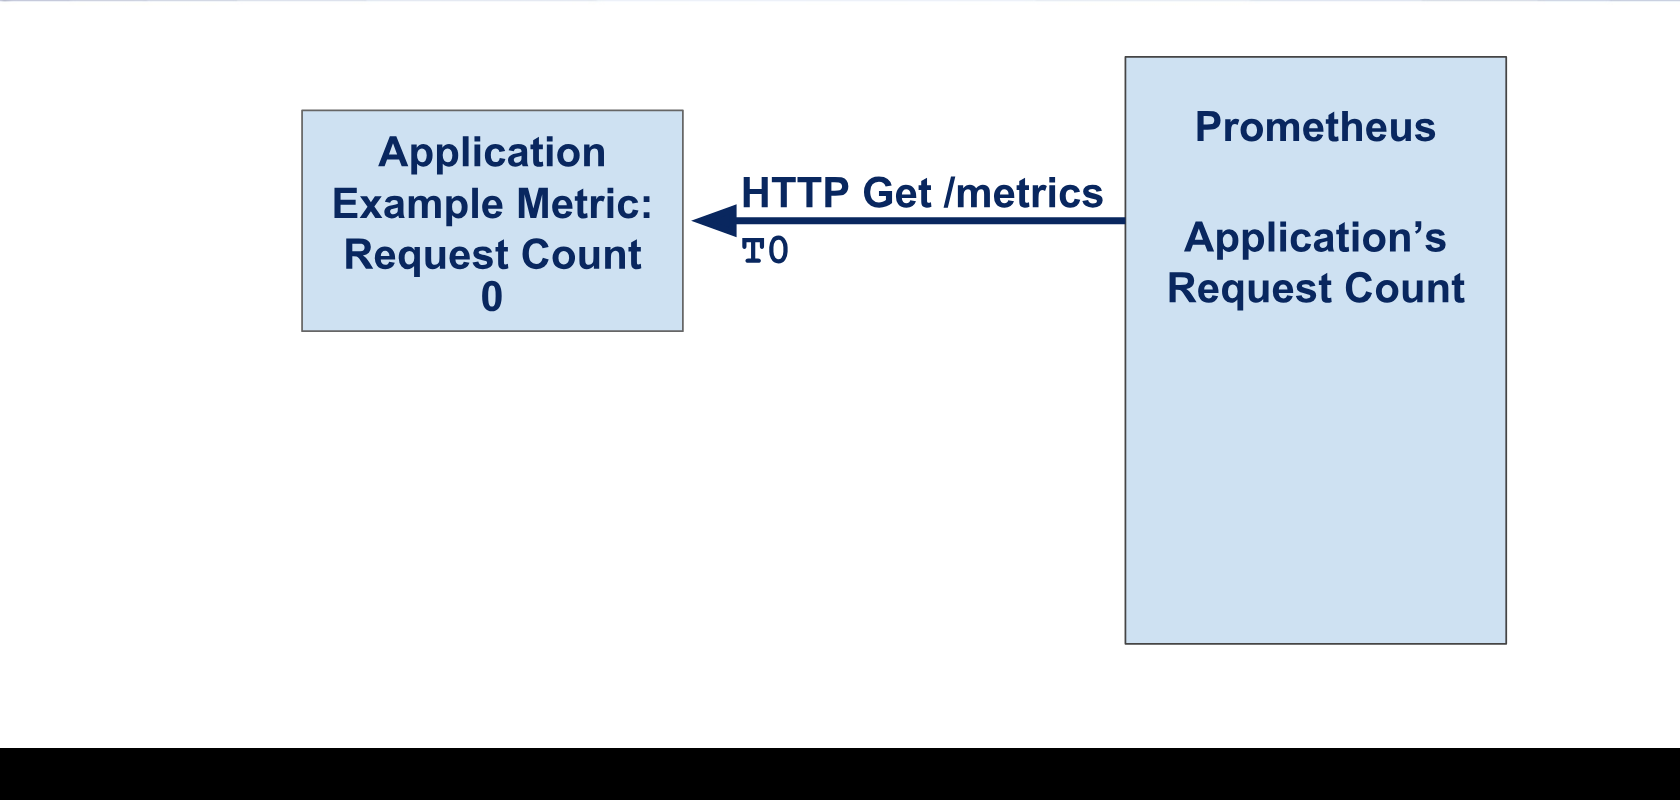
\includegraphics[width=\textwidth]{02-cropped.png}
\end{frame}

\begin{frame}
        \frametitle{Generating, scraping, and persisting times series}
        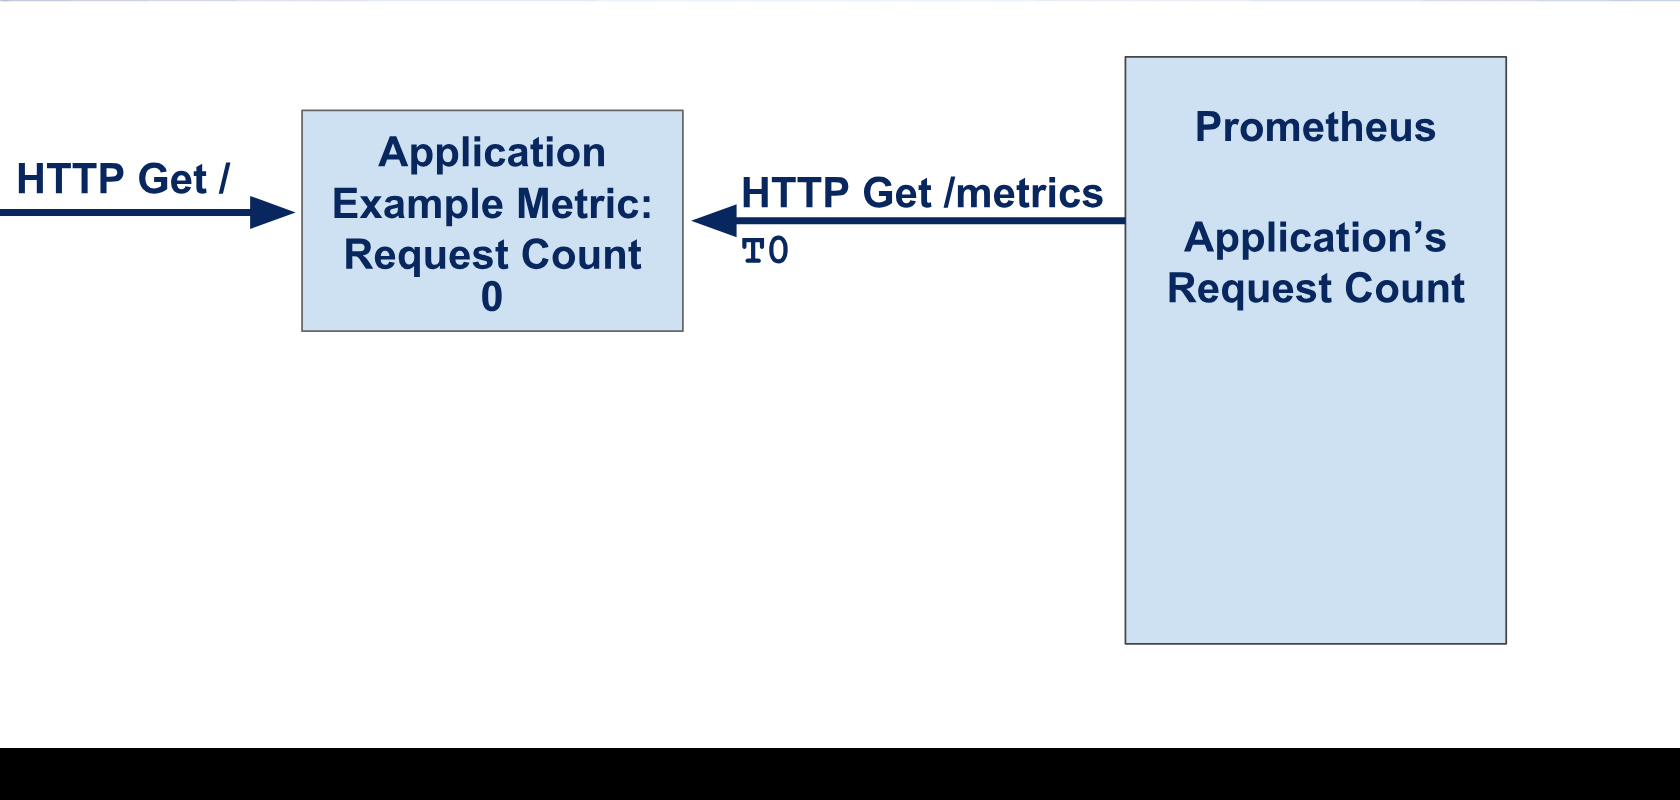
\includegraphics[width=\textwidth]{03-cropped.png}
\end{frame}

\begin{frame}
        \frametitle{Generating, scraping, and persisting times series}
        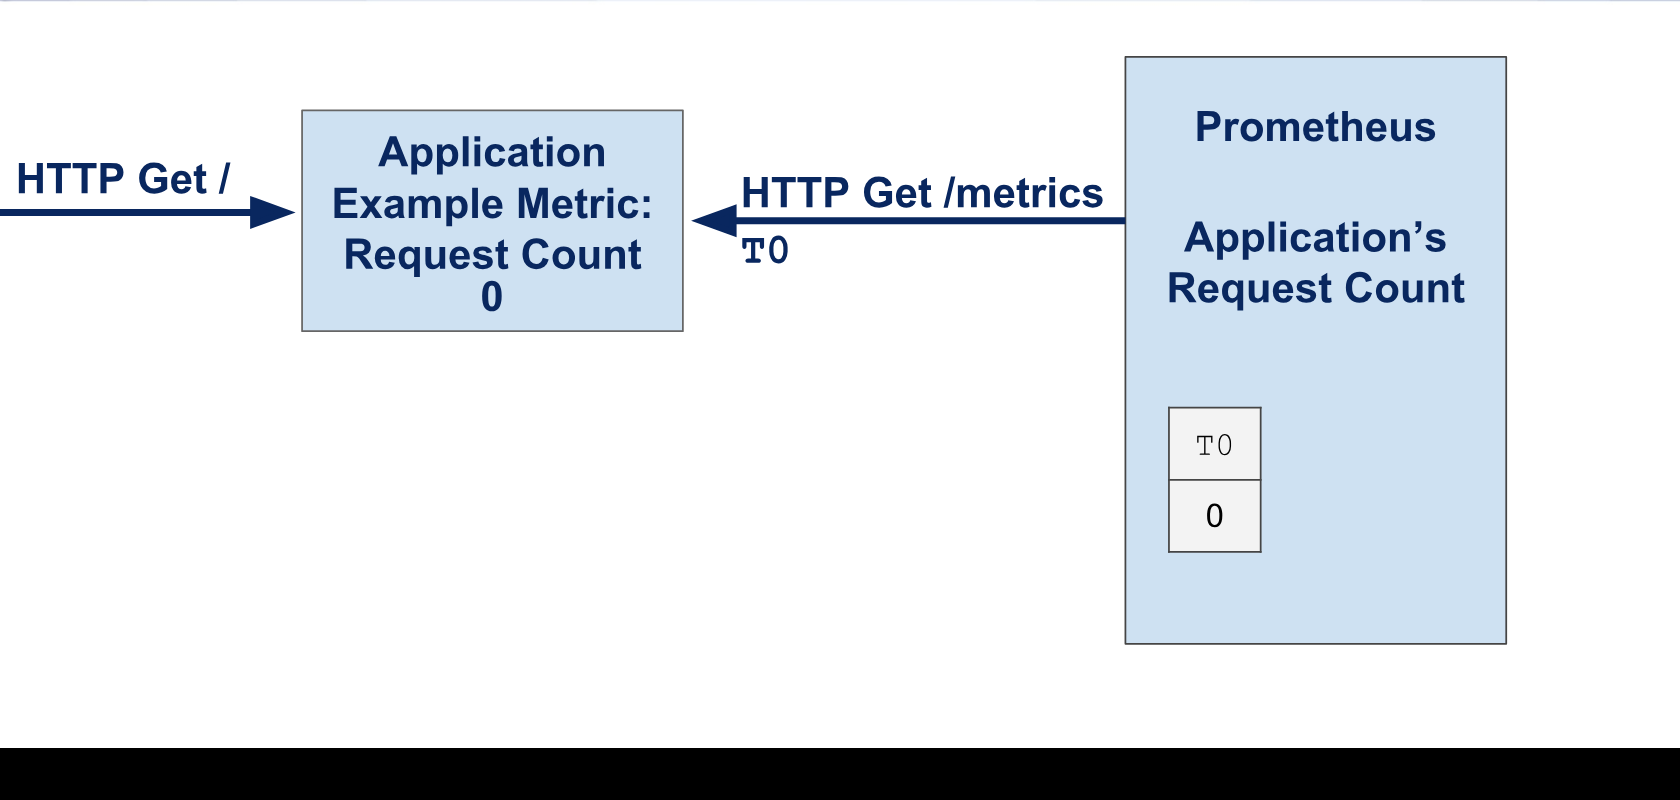
\includegraphics[width=\textwidth]{04-cropped.png}
\end{frame}

\begin{frame}
        \frametitle{Generating, scraping, and persisting times series}
        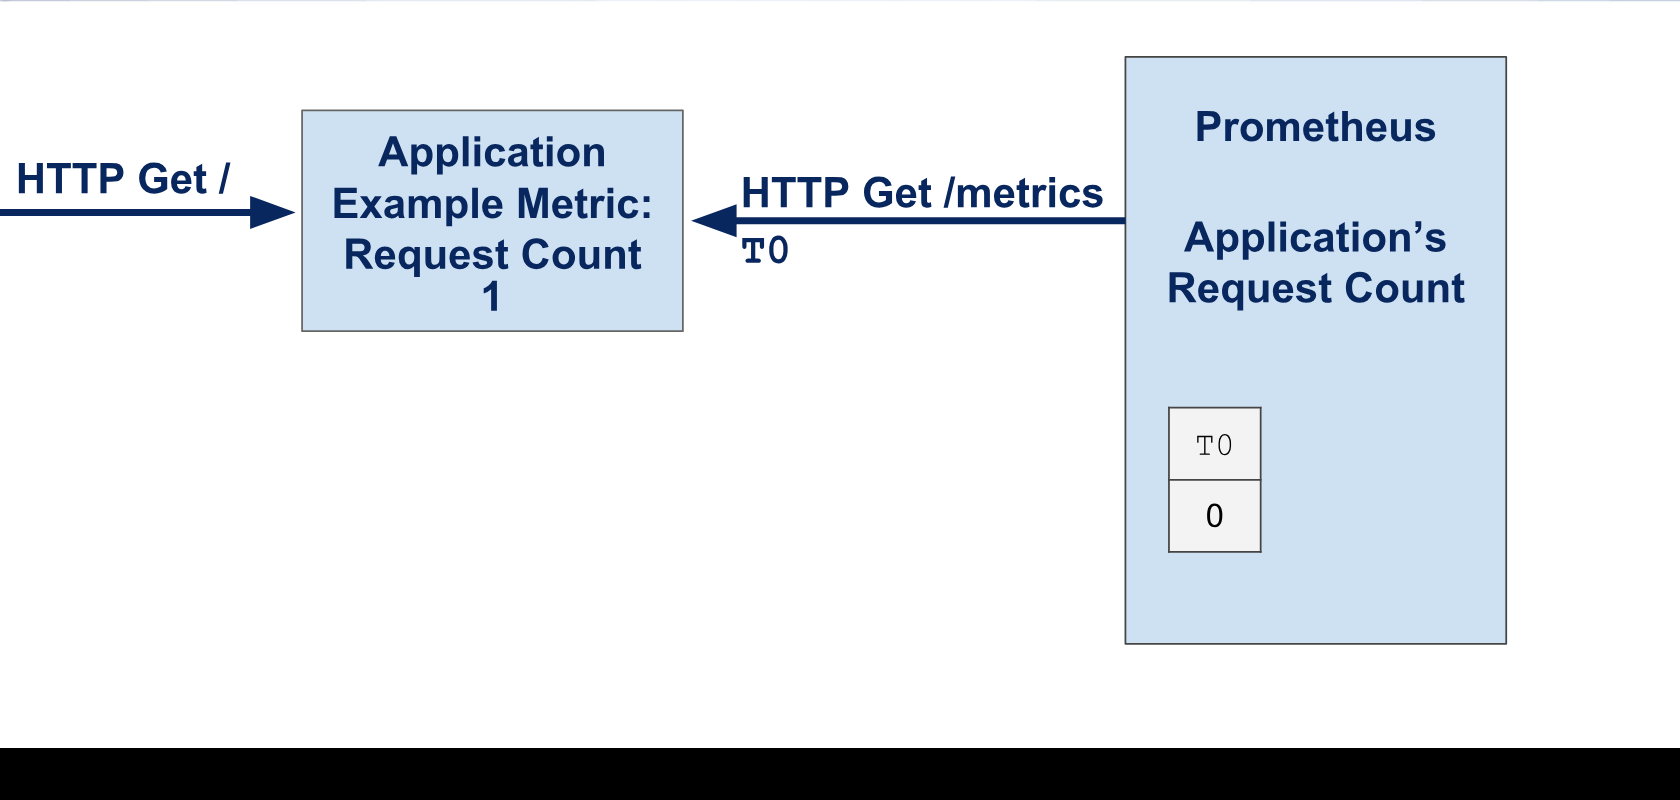
\includegraphics[width=\textwidth]{05-cropped.png}
\end{frame}

\begin{frame}
        \frametitle{Generating, scraping, and persisting times series}
        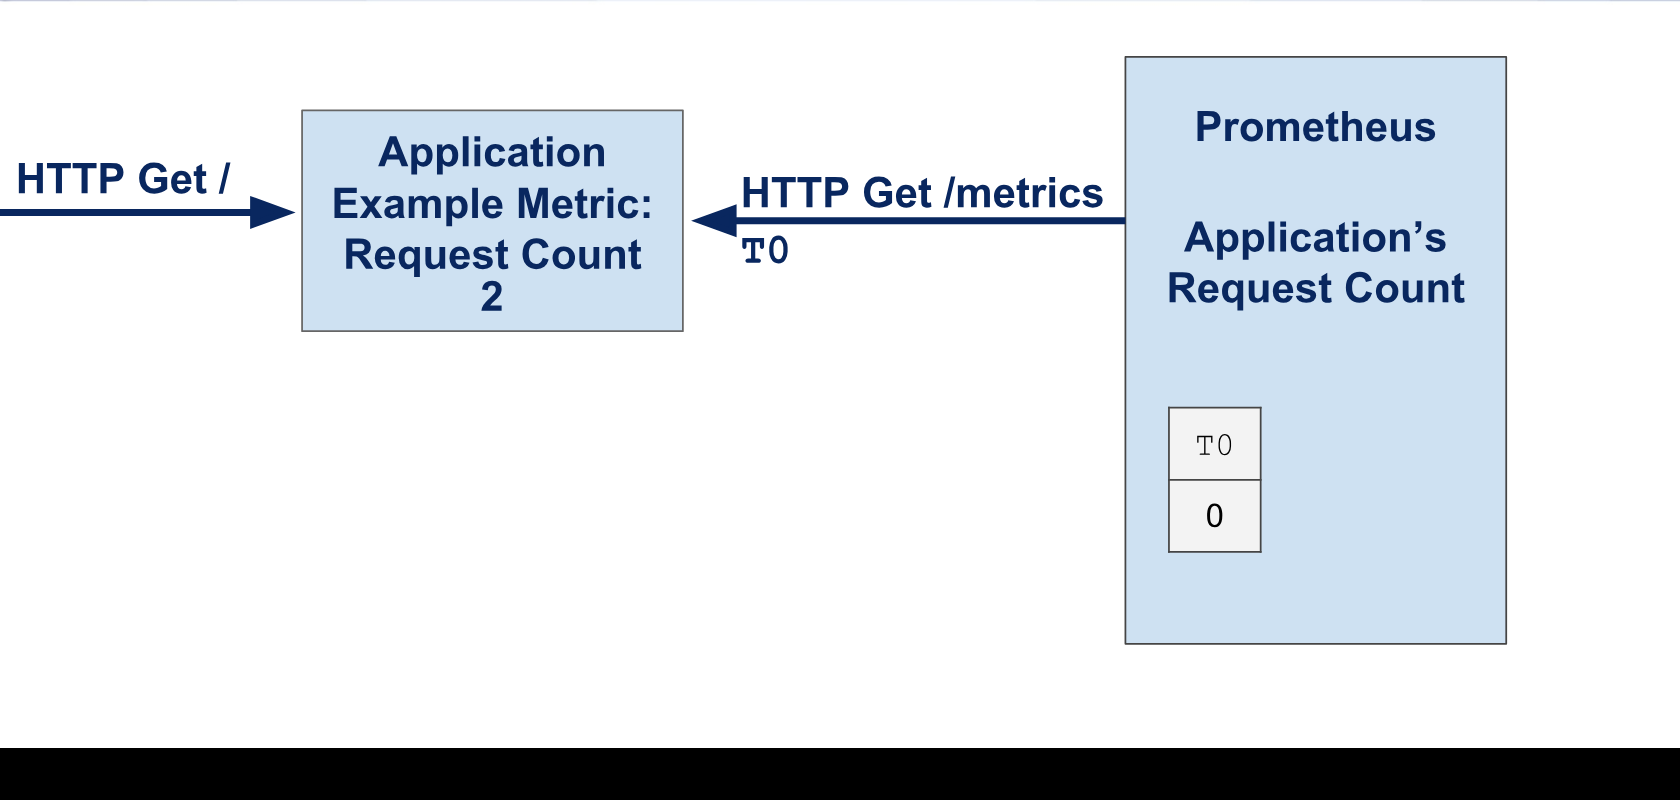
\includegraphics[width=\textwidth]{06-cropped.png}
\end{frame}

\begin{frame}
        \frametitle{Generating, scraping, and persisting times series}
        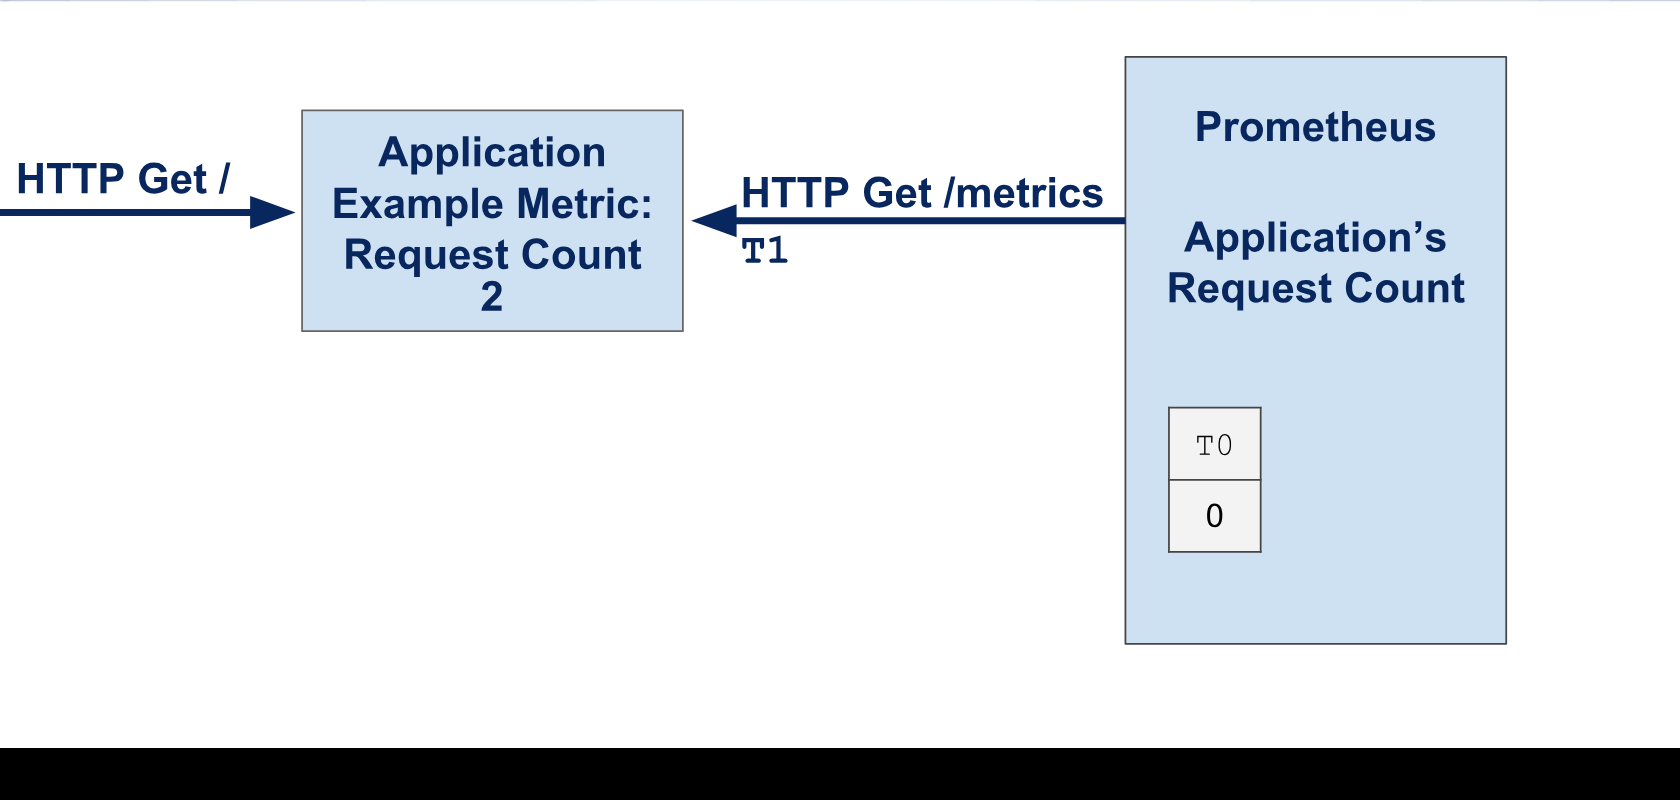
\includegraphics[width=\textwidth]{07-cropped.png}
\end{frame}

\begin{frame}
        \frametitle{Generating, scraping, and persisting times series}
        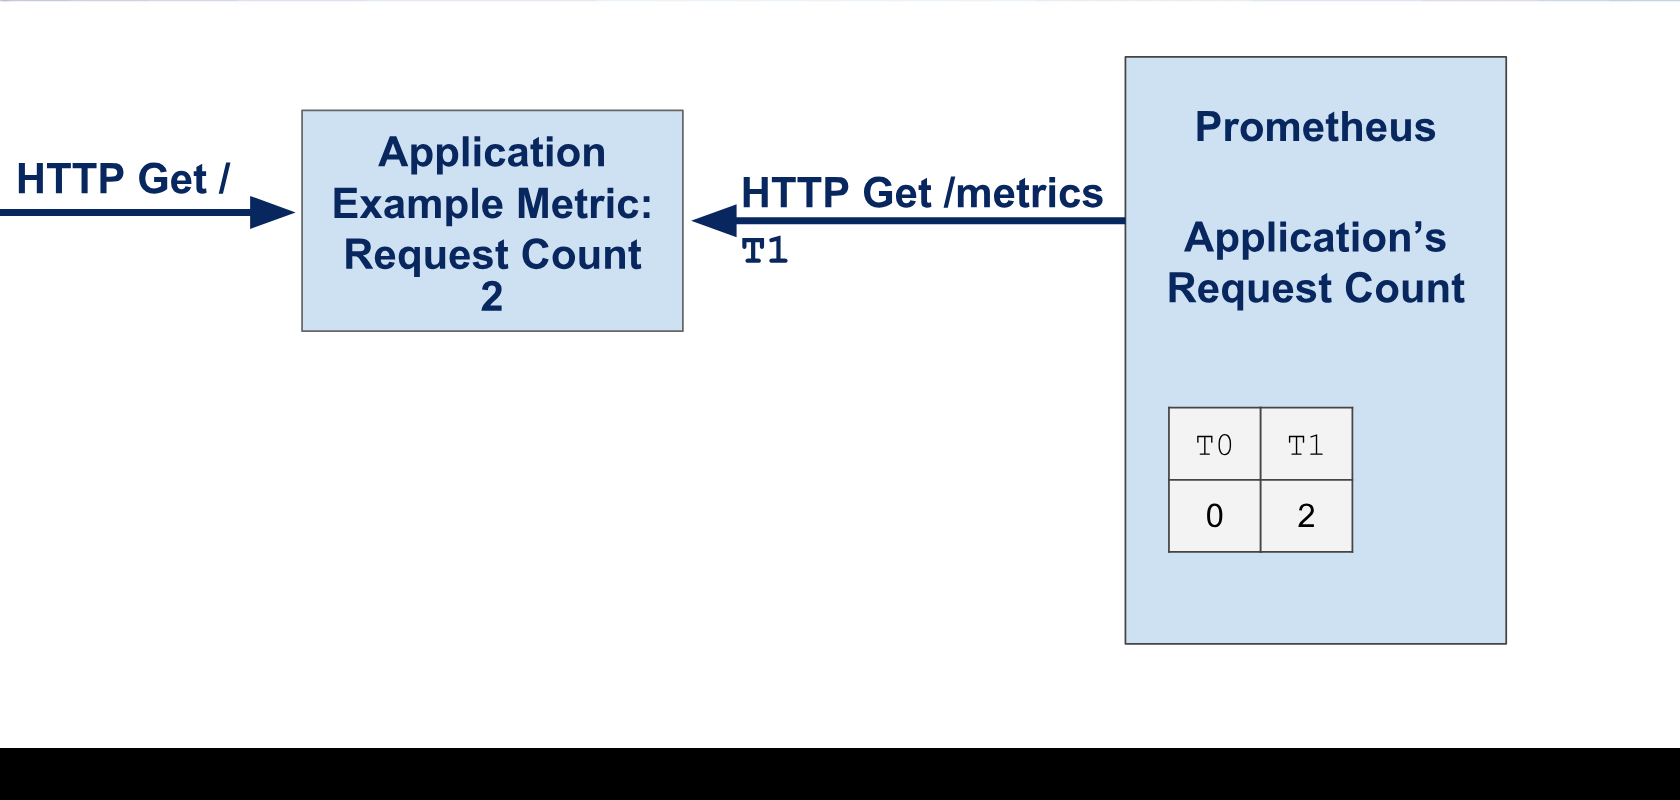
\includegraphics[width=\textwidth]{08-cropped.png}
\end{frame}

\begin{frame}
        \frametitle{Generating, scraping, and persisting times series}
        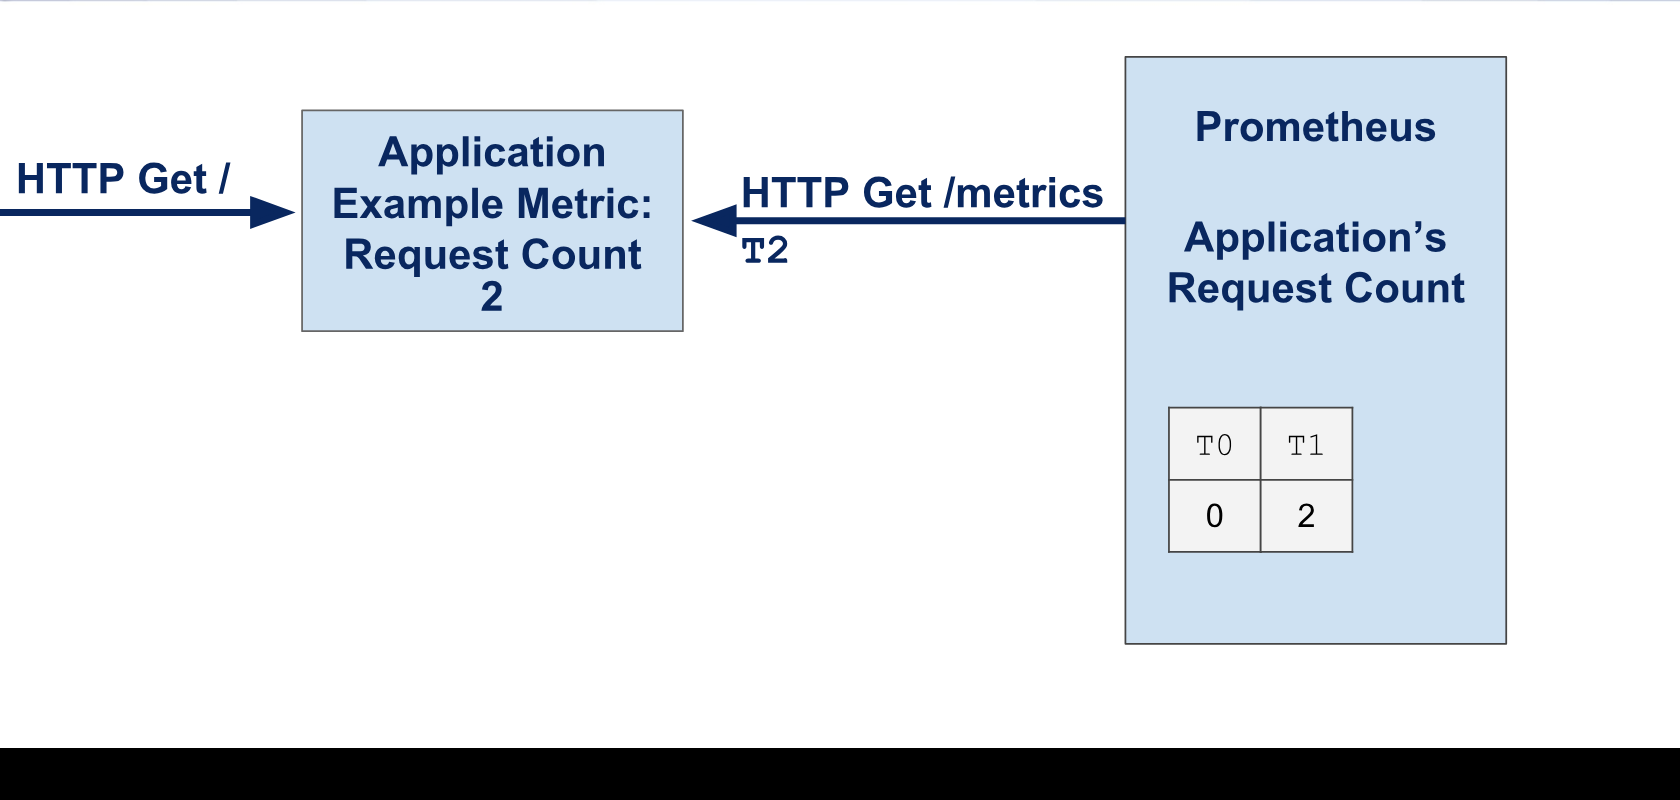
\includegraphics[width=\textwidth]{09-cropped.png}
\end{frame}

\begin{frame}
        \frametitle{Generating, scraping, and persisting times series}
        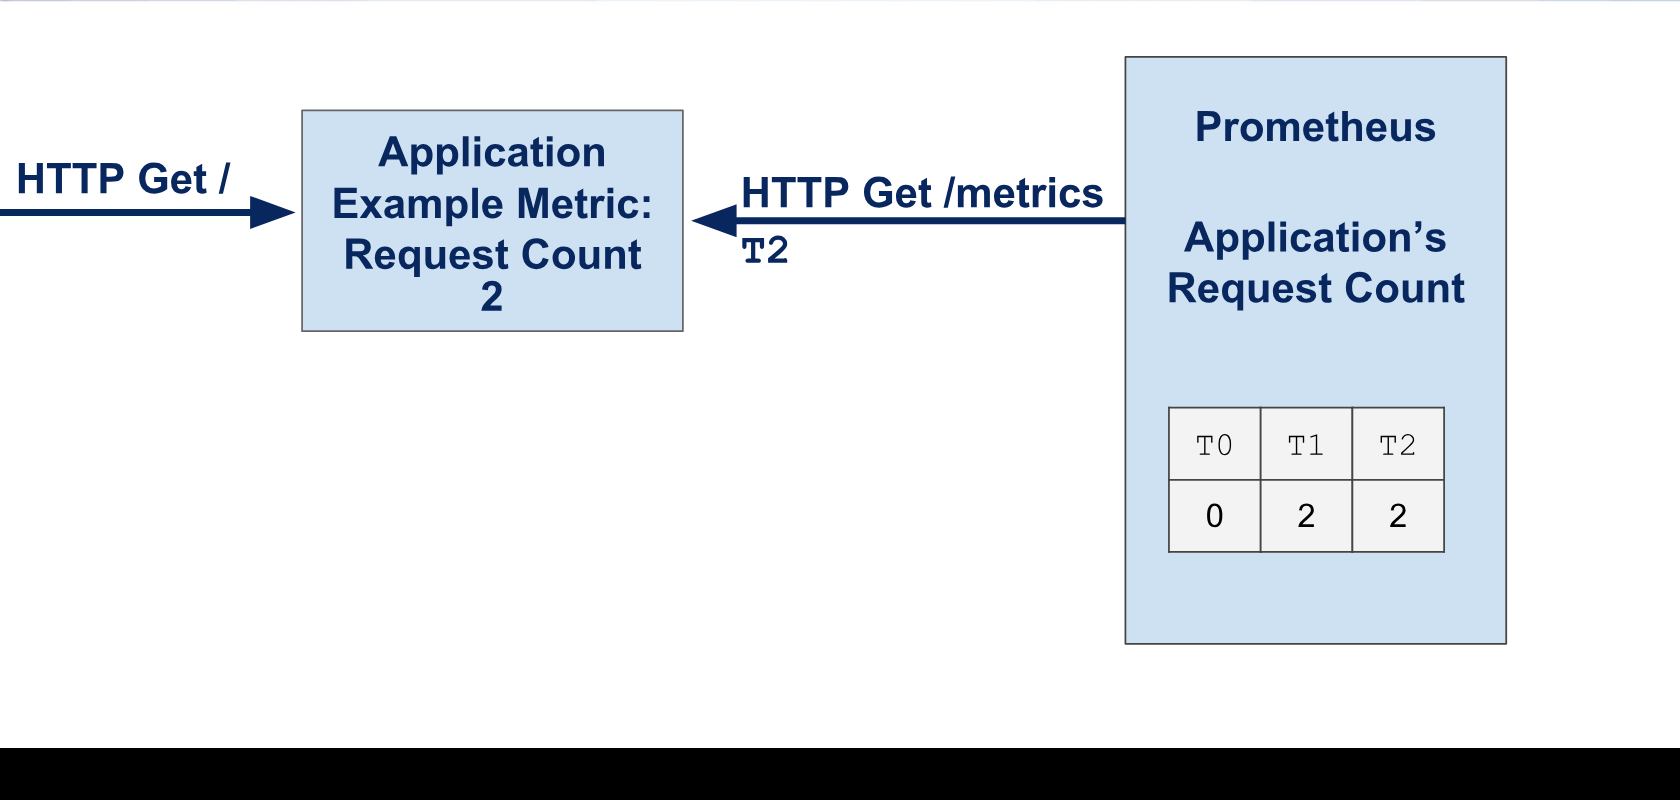
\includegraphics[width=\textwidth]{10-cropped.png}
\end{frame}

\begin{frame}
        \frametitle{Generating, scraping, and persisting times series}
        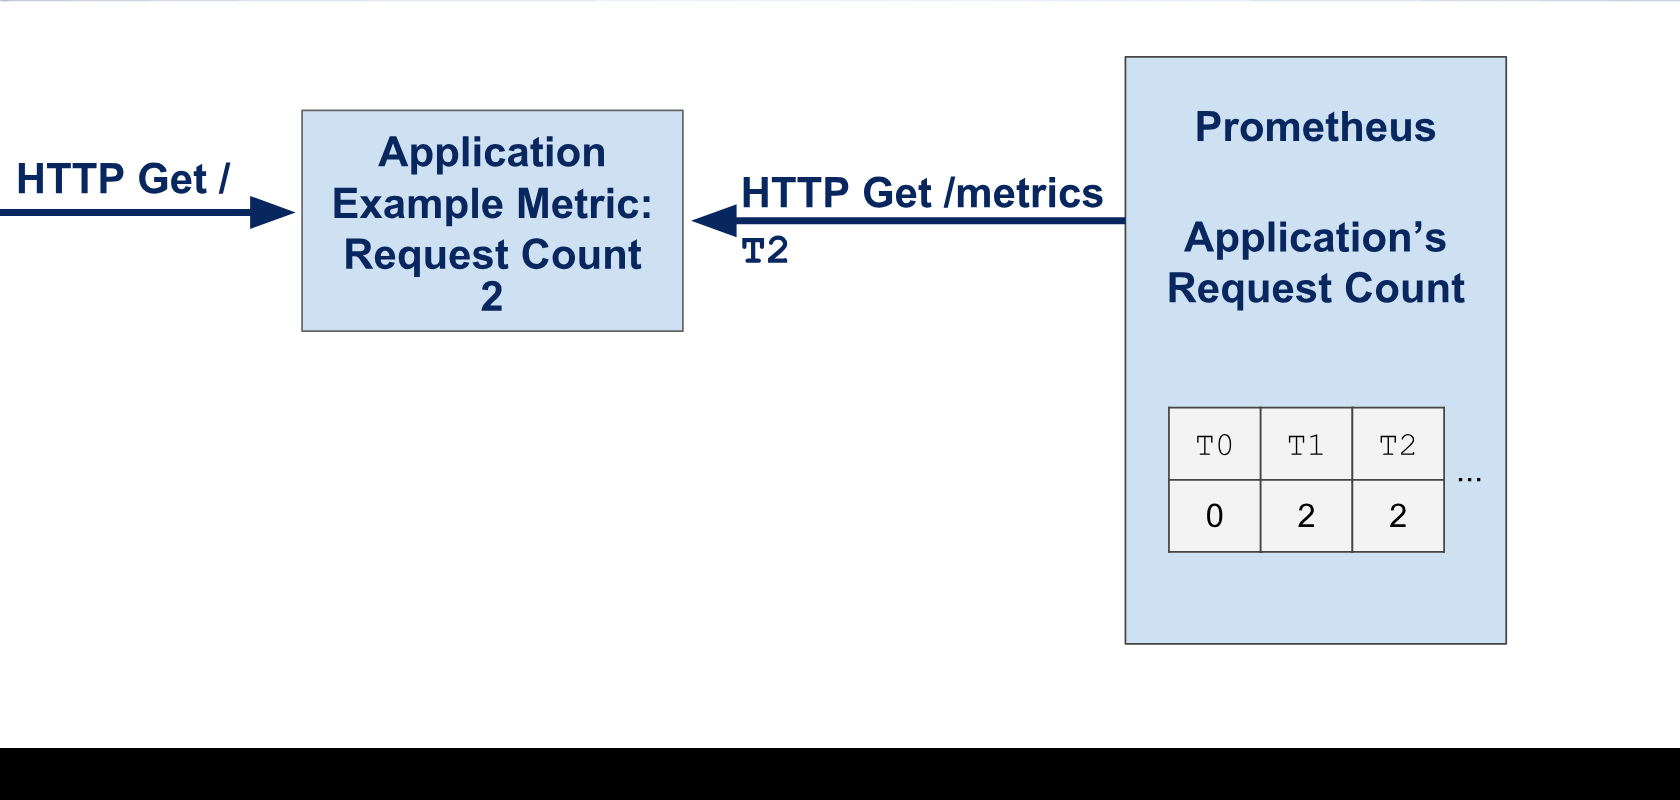
\includegraphics[width=\textwidth]{11-cropped.png}
\end{frame}


\subsection{}


\begin{frame}
	\frametitle{Main selling points}
	\begin{itemize}
		\item Highly dynamic, built-in service discovery
		\item No hierarchical model, n-dimensional label set
		\item PromQL: for processing, graphing, alerting, and export
		\item Simple operation
		\item Highly efficient
	\end{itemize}
\end{frame}

\begin{frame}
	\frametitle{Working assumptions \& concepts}
	\begin{itemize}
		\item Prometheus is a pull-based system
		\item Black-box monitoring: Looking at a service from the outside (Does the server answer to HTTP requests?)
		\item White-box monitoring: Instrumention code from the inside (How much time does this subroutine take?)
		\item Every service should have its own metrics endpoint
		\item Hard API commitments within major versions
		\item No built-in TLS yet, use reverse proxies for now
	\end{itemize}
\end{frame}

\begin{frame}
	\frametitle{Time series}
	\begin{itemize}
		\item Time series are recorded values which change over time
		\item Individual events are usually merged into counters and/or histograms
		\item Changing values are recorded as gauges
		\item Typical examples
		\begin{itemize}
			\item Access rates to a webserver (counter)
			\item Temperatures in a datacenter (gauge)
		\end{itemize}
	\end{itemize}
\end{frame}

\begin{frame}
	\frametitle{Efficiency}
	\begin{itemize}
		\item 1,000,000+ samples/second no problem on currect hardware
		\item 200,000 samples/second/core
		\item 16 bytes/sample compressed to 1.36 bytes/sample
		\item Cheap ingestion \& storage means more data for you
	\end{itemize}
\end{frame}

\begin{frame}[fragile]
	\frametitle{Exposition format}
	\fontsize{10pt}{12}\selectfont
	\begin{verbatim}
http_requests_total{env="prod",method="post",code="200"} 1027
http_requests_total{env="prod",method="post",code="400"} 3
http_requests_total{env="prod",method="post",code="500"} 12
http_requests_total{env="prod",method="get",code="200"} 20
http_requests_total{env="test",method="post",code="200"} 372
http_requests_total{env="test",method="post",code="400"} 75
	\end{verbatim}
\end{frame}

\begin{frame}[fragile]
	\frametitle{PromQL vs SQL}
	\fontsize{10pt}{12}\selectfont
	\begin{verbatim}
avg by(city) (temperature_celsius{country=”germany”})

SELECT city, AVG(value) FROM temperature_celsius WHERE \
 country=”germany” GROUP BY city

rate(errors{job=”foo”}[5m]) / rate(total{job=”foo”}[5m])

SELECT errors.job, errors.instance, […more labels…], \
 rate(errors.value, 5m) / rate(total.value, 5m) \
 FROM errors JOIN total ON […all label equalities…] \
 WHERE errors.job=”foo” AND total.job=”foo”
	\end{verbatim}
\end{frame}

\begin{frame}
	\frametitle{Grafana}
	\begin{itemize}
		\item Supports dozens of data sources
		\item Modern UI
		\item Allows for complex data manipulation and visualization
		\item Native Prometheus support
		\item New feature: Interactive exploration of Prometheus data
	\end{itemize}
\end{frame}

%TODO pics?
%\begin{frame}
%	\frametitle{Grafana}
%%	\includegraphics[width=0.8\textwidth,natwidth=1583,natheight=555]{power_usage.png}
%\end{frame}


\section{Operations \& observability}

\subsection{}

\begin{frame}
	\frametitle{Toil}
	"Toil is manual, repeated work with no lasting benefit which scales linearly with your service"
	\vfill
	\begin{itemize}
		\item If teams are busy firefighting, they don't have time to engineer
		\item Keep legacy systems working, but have clear path forward
		\item Keep extra effort on the team low, if possible
		\item Strive for immediate benefits
		\item Focus on removing repeated, manual tasks of no lasting benefit
		\item Show that you free up time and reduce toil
% operations stakeholders fear change
  % they get paid to keep the current system up and running, not to increase change
% everyone wants to live in a SRE world with error budgets and caps on toil
%Toil in too many places
	\end{itemize}
	\vfill
\end{frame}

\begin{frame}
	\frametitle{Sanity \& sleep}
	\begin{itemize}
		\item If it's not actionable, it's not an alert
		\item If it's not urgent, it's not an alert
		\item Important but non-urgent incidents are handled during business hours
		\item Predict your usage so you add capacity during business hours
		\item If there's no playbook, it does not go into production
		\item If a service does not have proper SLOs and alerts, it does not go into production
	\end{itemize}
\end{frame}

\begin{frame}
	\frametitle{Perspective \& Incentives}
	"An engineer can talk for hours about source code; try that with the CEO"
	\vfill
	\begin{itemize}
		\item Managers: revenue, process execution
		\item Architects: clean design, process definition
		\item Product/Service owners: Powerful dashboards
		\item Team leads: morale, quick execution
		\item Operators: reduce toil, increase sleep
%  Different parts of the picture for different people and languages
%  Anyone can talk to an engineer about a UPS for two hours, but management...
	\end{itemize}
	\vfill
	Tell everyone what they need to hear (but never lie)
	\vfill
\end{frame}

% money is made with brownfield so you need to make sure there is no impact
% lots of overlap until new stuff gains trust
% people's motivation is to resist change; and that's OK until the system can actually handle change
% most will readily agree that the new approach is better, but they fear the way there
% ideally, we should magic from zero to done without anyone noticing

\begin{frame}
	\frametitle{Post-Mortems}
	\begin{itemize}
		\item Mistakes happen
		\item It is important to learn from mistakes so not to repeat them
		\item To write a good incident report, there must be no fear of retribution
		\item Blame-free post-mortems allow everyone to document exactly what went wrong and in what order
		\item It is important to build trust among the teams and management
	\end{itemize}
\end{frame}

\begin{frame}
	\frametitle{Leverage}
	\begin{itemize}
		\item One combined system allows for correlation and combination
		\item Power usage against service load
		\item Optical networks against outside temperature
		\item Datacenter power feed load against new deployments
		\item ...and lots more
		\item Metrics are the starting point of most observability stories
	\end{itemize}
\end{frame}

\begin{frame}
	\frametitle{Oracle}
	\begin{itemize}
		\item One source of truth for
		\begin{itemize}
			\item Tactical overview for current state
			\item Dashboards for drill-down
			\item Auto-generated PDFs for customers
			\item Global SLO statements for sales
			\item Usage exports for accounting
		\end{itemize}
	\item If all you have is a hammer... choose your hammer well
	\end{itemize}
\end{frame}

%\begin{frame}
%	\frametitle{Caveat}
%	\begin{itemize}
%		\item In brownfield, revenue comes from legacy systems
%		\item If you impact revenue, all buy-in is gone
%	\end{itemize}
%\end{frame}





%Not all teams tracked and compared KPIs over time

%Dashboard
%Perpetual greenfield
%One tool fits all
%Make your hammer fit your nails

\section{Outro}

\subsection{}

\begin{frame}
	\frametitle{Thanks!}
		\begin{center}
			\vfill
			Thanks for listening!\\
			\vfill
			Questions?
			\vfill
%			See slide footer for contact info.
%			\vfill
		\end{center}
\end{frame}

\end{document}

%\begin{frame}
%	\frametitle{}
%	\begin{itemize}
%		\item 
%		\item 
%		\item 
%		\item 
%		\item 
%	\end{itemize}
%\end{frame}
